\chapter{مقایسه، آزمایش‌ها، و نتایج}
در این فصل به بررسی نتایج حاصل از پیاده‌سازی الگوریتم‌ها و مقایسه آن‌ها می‌پردازیم.
\section{ارزیابی الگوریتم‌ها}
در این بخش، میانگین پاداش، درصد رخداد هر یک از حالت‌های پایانی بازی (گل، بیرون رفتن از زمین،اتمام زمان، گرفتن دروازه‌بان)
و خطای میانگین مدل‌ها را در طی زمان یادگیری ارزیابی کرده،
سپس بهترین مدل هر الگوریتم‌ را با هم مقایسه می‌کنیم.
\section{مقایسه سرعت یادگیری با گسسته سازی‌ها متفاوت}
مقایسه تقسیم‌بندی‌های متفاوت قدرت و تعداد زوایای ممکن، و حالت پیوسته.
\section{بررسی تعمیم پذیری}
در این بخش، با تست علیه دروازه‌بان تیم‌هایی که مقابل آن‌ها یادگیری رخ نداده، می‌بینیم که آیا این یادگیری تعمیم‌پذیر بوده یا خیر.
\section{بررسی تاثیر استفاده از تابع پاداش هوشمند‌تر}
عامل در ابتدای یادگیری، هنوز به درک اینکه در چه حالتی می‌تواند شوت منجر به گل داشته باشد نرسیده است.
از آنجا که این عمل با عمل رسیدن به موقعیت شوت‌زنی متفاوت است، عامل ممکن است دیر به دیر به حالت‌هایی که شوت زدن در آن ممکن است برسد.
بنابرین در حین یادگیری نسبت به ضربه با سرعت‌های بالا بدبین می‌شود.

از این رو می‌توان پاداش مثبتی برای حالتی که عامل زاویه و سرعت مناسبی برای شوت دارد، ولی شوت نزده است، در نظر گرفت.
این تغییر باعث تشویق عامل به کاوش بیشتر این حالت‌ها میشود، چرا که در غیر این صورت باید کاملا تصادفی به حالت گل می‌رسید.
یک مثلث بین توپ و تیرک‌های دروازه رسم می‌کنیم. در صورتی که هیچ بخشی از دروازه‌بان در ناحیه این مثلث نباشد، پاداش مثبتی به عامل می‌دهیم؛ چرا که در این حالت به احتمال بالا می‌توانیم بعد از چند گام به گل برسیم.
\begin{figure}
    \centering
    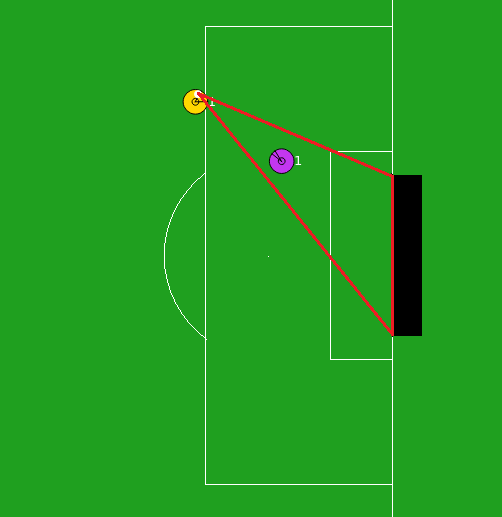
\includegraphics[width=0.5\textwidth]{images/bonus_reward.png}
    \caption{مثلث بین توپ و تیرک‌های دروازه، که در صورت عدم وجود دروازه‌بان در آن، پاداش مثبتی به عامل داده می‌شود.}
    \label{fig:shot_reward}
\end{figure}

\section{تسریع یادگیری با تلفیق با رفتار سطح بالای شوت}
همانطور که در بخش قبلی گفتیم، چالش یادگیری این محیط در واقع هم رسیدن به موقعیت شوت‌زنی، و هم شوت زدن است.
بنابراین می‌توانیم از یک مدل دیگر برای تشویق عامل به شوت زدن استفاده کنیم.
یک عمل خاص مدنظر می‌گیریم که در صورت انتخاب شدن توسط عامل، شوت کد پایه \lr{Agent2D} 
انجام می‌شود. این کد در صورت وجود شوت ممکن، آن را انجام می‌دهد و در غیر این صورت، هیچ عملی انجام نمی‌شود.
در صورتی که عامل این عمل را انتخاب کند ولی به گل نرسد، پاداش منفیی به آن داده می‌شود، تا عامل استفاده صحیح از این ابزار را یاد بگیرد.
%%%%%%%%%%%%%%%%%%%%%%%%%%%%%%%%%%%%%%%%%%%
% در بخش پایانی گزارش، جمعبندي و مروري بر سیر مطالب عنوان شده در گزارش خواهیم داشت. همچنین نتایج حاصل را بیان
% کرده و پیشنهادهایی براي ادامه کار در این موضوع ارائه میدهیم.
% \section{نتیجه‌گیری}
% این گزارش ۶ الگوریتم‌ برای پیش‌بینی مصرف انرژی ساختمان‌ها را مورد بررسی قرار داد که برای این الگوریتم‌ها داده‌های مصرف آینده‌ی ساختمان‌ها و مصرف گذشته‌شان موجود بود. 
% همچنین در این مقاله اهمیت برخی متغیرها مانند وضعیت دمای محیط و تعداد ساکنین ساختمان در هر زمان نیز مورد توجه قرار گرفتند و اهمیت آن‌ها در تصمیم گیری مشخص گردید.
% چندین مدل یادگیری ماشین موفق با استفاده از داده‌های انرژی ثبت‌شده گذشته برای پیش‌بینی کوتاه‌مدت، میان‌مدت و بلندمدت توسعه یافته‌اند. مشاهده می شود 
% که هر یک از تکنیک های توصیف شده دارای مجموعه ای از مزایا و معایب است. اینها با توجه به تجزیه و تحلیل داده های انرژی ساختمان به تفصیل تجزیه و تحلیل و ارائه شده اند.
%  تأکید ویژه بر مدل ترکیبی داده شده است، که ترکیبی از دو یا چند تکنیک یادگیری ماشینی است به نحوی که هر مدل قدرت دیگری 
%  را تحسین می کند. به عنوان مثال، یک مدل ترکیبی که میانگین متحرک خودهمبسته یکپارچه و الگوریتم‌های تکاملی را در نظر می‌گیرد، می‌تواند
%   از مدل میانگین متحرک خودهمبسته یکپارچه برای تعیین تناوب و خطی بودن استفاده کند، در حالی که الگوریتم‌ تکاملی می‌تواند به طور موثر باقیمانده‌ها را تعیین کند. ترکیبات مختلفی از مدل ترکیبی و تازگی آنها در
%    ادبیات شناسایی شده و به طور سیستماتیک در این مقاله ارائه شده است. مشاهده می‌شود
%    که ترکیب تکنیک‌های پیش‌بینی سری‌های زمانی مانند شبکه ی عصبی مصنوعی، میانگین متحرک خودهمبسته یکپارچه به خوبی با 
%    تکنیک‌های بهینه‌سازی ترکیب می‌شوند. چنین ترکیب‌هایی به طور گسترده در تحقیقات اختصاص یافته به بهینه‌سازی ساختمان مورد بررسی قرار گرفته‌اند.
%     انتظار می رود روند رو به رشد
%     در تحقیقات در بهره وری انرژی ساختمان در پرتو انگیزه پایداری جهانی ادامه یابد. این امر نظارت و پیش بینی داده های انرژی در 
%     زمان واقعی را در این زمینه مرتبط و حیاتی می کند. این مقاله خلاصه‌ای جامع از تکنیک‌های پیش‌بینی موجود همراه با ترکیبی
%      از مدل ترکیبی ارائه می‌کند و راه را برای تحقیقات آینده در زمینه مصرف انرژی ساختمان هموار می‌کند.
%      \\
%      حوزه بهینه سازی ساختمان بر اساس یک شبکه گسترده جمع آوری داده، نظارت، پیش بینی، بهینه سازی و کنترل است. تمام این زیرساخت‌ها
%       همواره به کل هزینه عملیاتی ساختمان می‌افزایند. چالش در اینجا بررسی مزایای اضافه شده از نظر هزینه سرمایه گذاری و هزینه به دست آمده
%       به دلیل صرفه جویی در انرژی ناشی از بهینه سازی ساختمان است. مطالعات کمی وجود دارد که بخش مالی را برای کنترل عملکرد و بهینه سازی ساختمان 
%      برجسته می کند. این محدودیت در به اشتراک گذاری داده های هزینه یا به دلیل 
%      نیروهای بازار درگیر است یا به دلیل محرمانه بودن ماهیت داده های درگیر. لبی الدان\LTRfootnote{Labeodan} 
%      و همکاران. کاربردهای شبکه حسگرها و محرک‌های بی‌سیم کم‌هزینه را برای مدل‌سازی اشغال و کنترل روشنایی در یک ساختمان
%       اداری مورد بحث قرار داد \cite{labeodan2016application}. هزینه کل سیستم تقریبا 2575 یورو برای 12 ایستگاه کاری بود که
%       شامل حسگرهای حرکتی بی سیم و سنسورهای صندلی بود. نتایج نشان می دهد که به طور متوسط 24\% کاهش در مصرف انرژی روشنایی برای یک دوره
%       دو هفته ای با هزینه اجرا شده در حدود 215 یورو برای هر ایستگاه کاری است. نویسندگان خاطرنشان کردند که هزینه اولیه بالاتر و عدم آگاهی از عوامل مؤثر
%       در کاهش سرعت استقرار حسگرها هستند. با این حال، صرفه جویی در انرژی به دست آمده، سهولت استقرار و بهبود سنجش محیطی این
%       را به عنوان یک راه حل مناسب برای دستیابی به عملکرد بهبود 
%       یافته ساختمان نشان می دهد. کومار و همکاران همچنین متوجه شد که هزینه سنسورهای نظارت کنترل کیفیت هوای داخلی الزامات استقرار در مقیاس بزرگ برای کنترل و اتوماسیون را
%        برآورده نمی کند \cite{kumar2016real}. لیلیس و همکاران اشاره کنید
%        که علاقه به راه‌حل‌های 
%       مبتنی بر اینترنت اشیا\LTRfootnote{Internet Of Things (IOT)} مدرن برای بهینه‌سازی ساختمان به دلیل عدم برآورد منافع هزینه، مهار شده است \cite{lilis2017towards}. چن و همکاران اشاره کرد
%        که هزینه مربوط به مصرف انرژی مجموعه تصادفی ساختمان‌ها در چین با سیستم های اتوماسیون ساختمان تقریبا دو برابر ساختمان های
%        بدون سیستم اتوماسیون ساختمان است \cite{chen2016cost}. این به دلیل نقص سنسور و نقص استراتژی کنترل است که منجر به افزایش قابل توجهی در مصرف انرژی نهایی می شود.
%         \\
%         چند مطالعه مروری شبکه حسگر بی سیم را پوشش داده است که سیستم مدیریت انرژی ساختمان را برای کاربردهای خانه/ساختمان 
%         هوشمند فعال کرده است \cite{kazmi2014review,kuzlu2015review}. از آنجایی که فناوری کنترل پیش‌بینی مدل هنوز در مرحله توسعه است و 
%         نیاز به بهینه‌سازی سنگین بر اساس نوع و عملکرد ساختمان دارد،
%          پیاده‌سازی در حال حاضر بیشتر بر روی بستر آزمایشی و اعتبارسنجی تمرکز دارد. در عین حال، این فناوری هنوز
%          با هزینه لازم برای استقرار در مقیاس های بزرگ در دسترس نیست. 
%          این چالش ها منجر به نفوذ آهسته اتوماسیون ساختمان و بهینه سازی در کل می شود. دامنه این مقاله مروری، با این حال
%         ، محدود به مطالعه تکنیک‌های پیش‌بینی سری‌های زمانی برای مصرف انرژی ساختمان است که بخشی جدایی‌ناپذیر
%          از فرآیند بهینه‌سازی و کنترل ساختمان است.
% \section{پیشنهادها}
%     به طور کلی الگوریتم‌های هوش‌ مصنوعی که در زمینه‌ی پیش‌بینی سری داده‌های زمانی کار میکنند و بخش عمده‌ی آن‌ها که الگوریتم‌های یادگیری ماشین می‌شوند مشکلات و سختی‌های مخصوصی دارند
%     از جمله محدودیت‌های مربوط به یادگیری‌آن‌ها که نیازمند داده‌های بسیتر زیاد برای یادگیری و آموزش میباشد و هم‌چنین نیاز به توان پردازشی بالای آن‌ها که از جمله مشکلات روش‌های هوش مصنوعی 
%     به طور کلی میباشد. 
%     برای حل این مشکل پیشنهاد میشود که الگوریتم‌های نوینی با استفاده از روش‌های ترکیبی توسعه داده بشوند که نیاز به داده‌های زیاد برای یادگیری در آن‌ها کمتر باشد و بتوانند با شبیه‌سازی 
%     آموزش ببینند و همچنین برای حل مشکل پردازش‌های سنگین با تحقیقات جدید به سمت برخط کردن یادگیری الگوریتم‌های هوش مصنوعی حرکت بکنیم به این صورت که تمام پردازش‌های مورد نیاز 
%     الگوریتممان برروی سرورهای قدرتمندی در سطح منطقه انجام بشوند و ساختمان‌ها مشکل پردازشی‌شان از این نظر مرتفع بشود و تنها برای انجام اندازه‌ی مشخصی از پردازش برروی شبکه ی قدرتمندمان 
%     هزینه پرداخت کنند تا هزینه‌هایشان کاهش پیدا بکند.